\section{Implementasi}

Bagian ini akan menjelaskan tentang implementasi sistem kontrol adaptif secara terperinci.

\subsection{Batasan Implementasi}
Berikut adalah batasan yang ditetapkan dalam melakukan implementasi sistem kontrol adaptif.
\begin{enumerate}
    \item Masih menerapkan sistem \textit{single node} dan \textit{single pod}.
    \item Tidak memperhatikan optimalisasi dari model ARIMA.
    \item Hanya dapat menangani metrik yang sudah ditentukan, yaitu \textit{throughput} dari setiap operasi \textit{Elastic Search} serta utilisasi prosesor hingga memori.
    \item Tidak mempertimbangkan besarnya model seiring bertambahnya data.
    \item Komponen \textit{Metrics Fetcher} berjalan di proses lain dan diimplementasikan dalam \textit{script} yang berbeda dikarenakan bahasa Python memiliki kekurangan dalam penanganan \textit{multithreading}.
    \item Pertukaran data antara komponen \textit{Metrics Fetcher} dan \textit{Predictor} melalui stream file.
\end{enumerate}

\subsection{Kakas yang Digunakan}
Dalam melakukan implementasi ini diperlukan beberapa kakas, diantaranya adalah sebagai berikut.
\begin{enumerate}
    \item \textit{Docker}, \textit{Docker Desktop} dan \textit{Docker Desktop Kubernetes} untuk dipakai sebagai \textit{containerization} dan \textit{cluster} kubernetes lokal.
    \item Pandas dan Numpy untuk keperluan \textit{data processing} serta bentuk data untuk dikirimkan ke komponen lain serta model prediksi ARIMA.
    \item \textit{Kubernetes Python Client} untuk mengontrol \textit{cluster} kubernetes melalui kode Python.
    \item \textit{Pickle} untuk menyimpan model ARIMA sehingga persisten meskipun sistem di-\textit{restart}.
    \item \textit{Statsmodels} dan \textit{pmdarima} untuk membangun model ARIMA serta melakukan otomasi pencarian orde atau lebih dikenal sebagai Auto-ARIMA.
\end{enumerate}

\subsection{Persiapan \textit{Pods Elastic Search}}

Sebelum melakukan implementasi, diperlukan untuk menyalakan \textit{Pods Elastic Search}. Konfigurasi ini dilakukan dengan cara membuat \textit{file deployment}, contoh dapat dilihat pada gambar \ref{fig:spek-deployment}.

\begin{figure}[h]
    \centering
    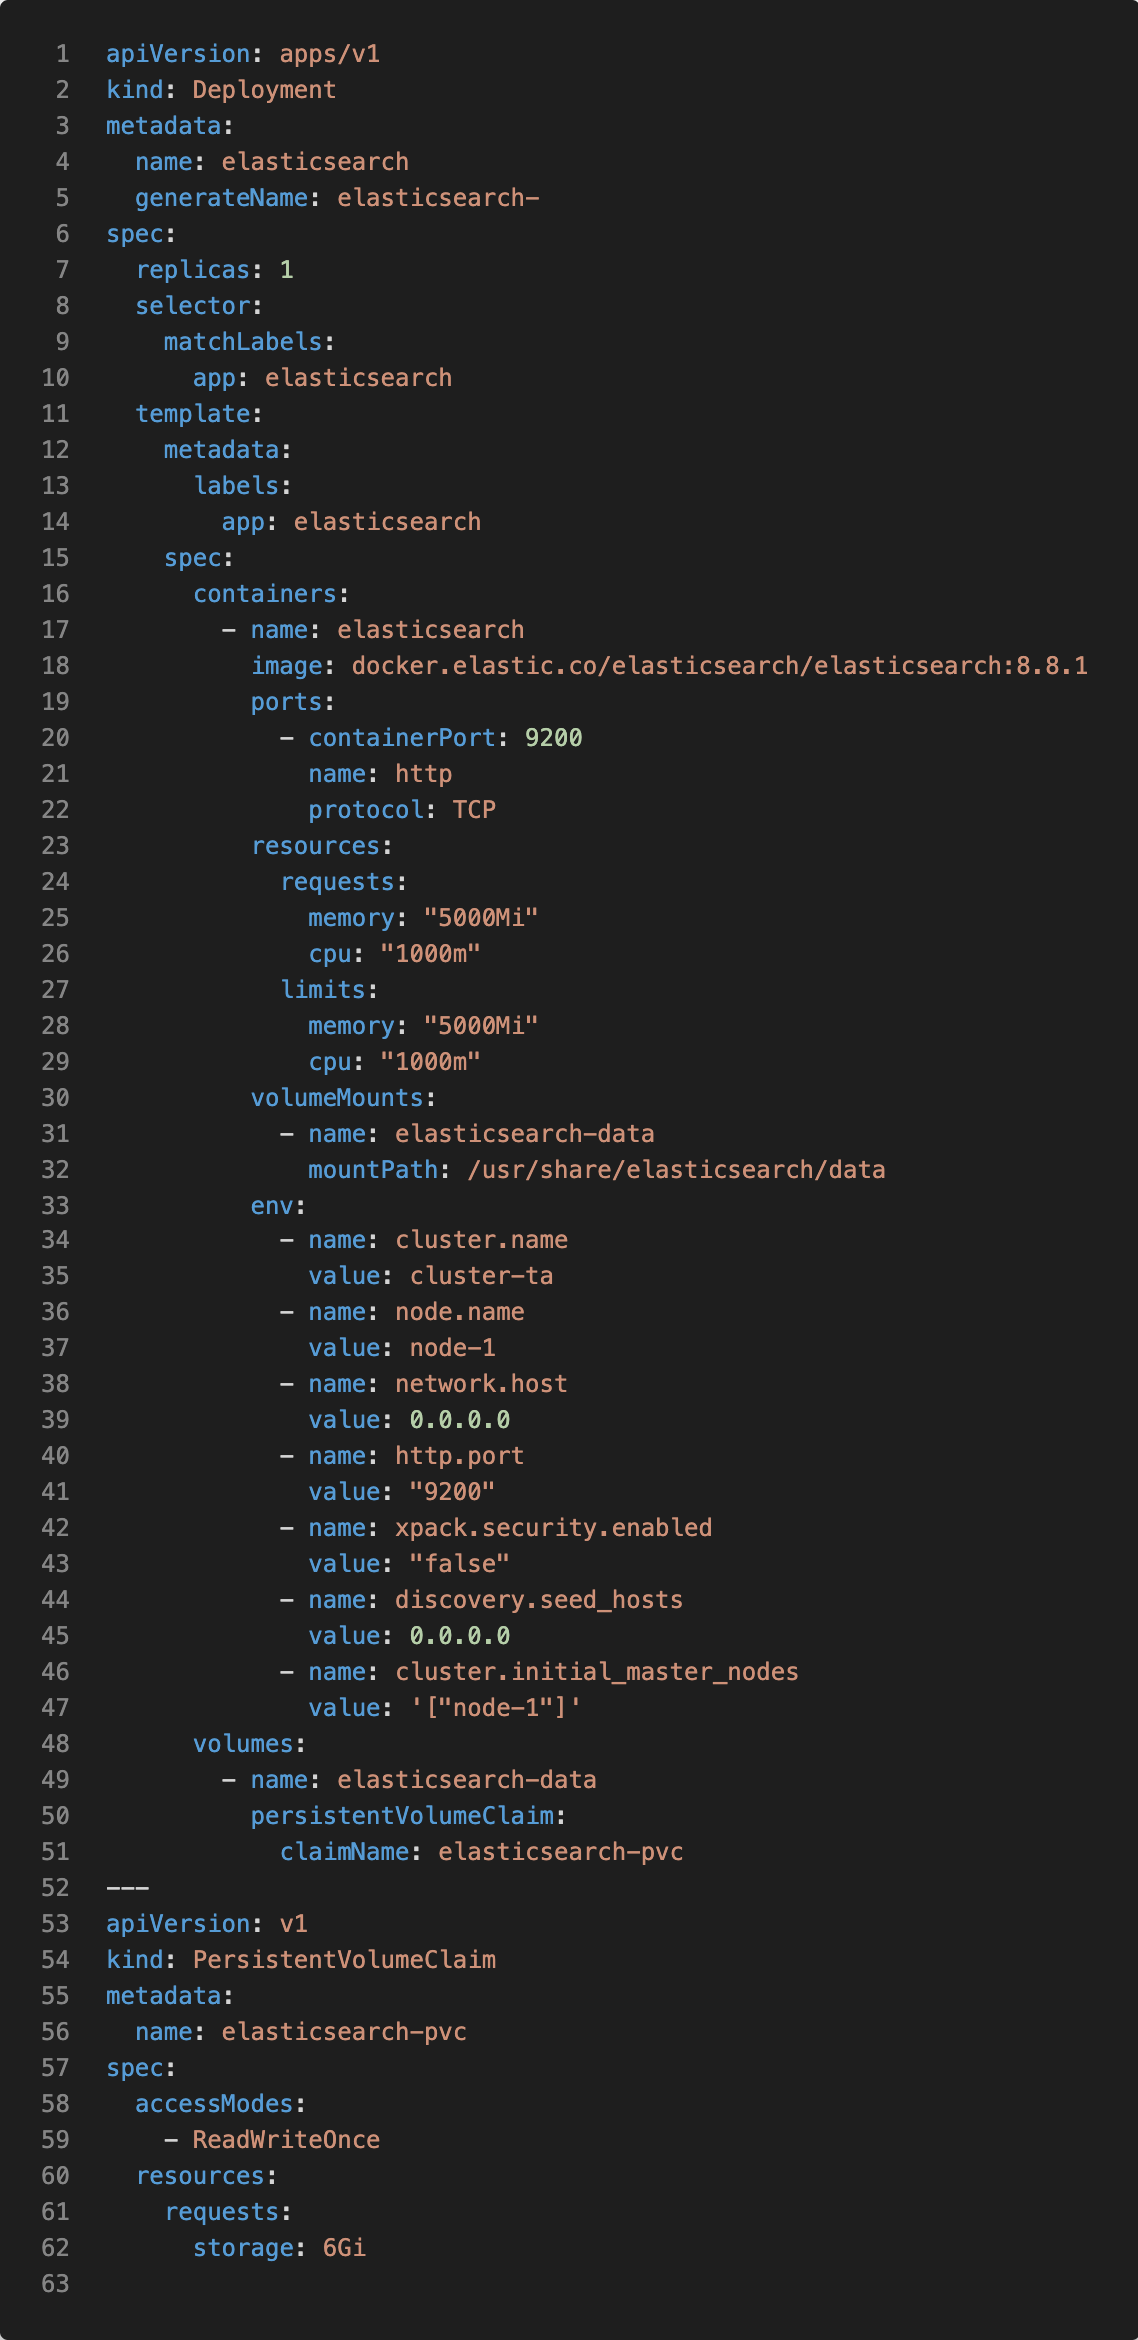
\includegraphics[width=0.75\textwidth]{chapter-4/spek-deployment.png}
    \caption{Konfigurasi \textit{Pods Elastic Search}}
    \label{fig:spek-deployment}
\end{figure}